\documentclass{article} % For LaTeX2e
\usepackage{nips14submit_e,times}
\usepackage{amsmath}
\usepackage{amsthm}
\usepackage{amssymb}
\usepackage{mathtools}
\usepackage{hyperref}
\usepackage{url}
\usepackage{algorithm}
\usepackage[noend]{algpseudocode}
%\documentstyle[nips14submit_09,times,art10]{article} % For LaTeX 2.09

\usepackage{graphicx}
\usepackage{caption}
\usepackage{subcaption}

\def\eQb#1\eQe{\begin{eqnarray*}#1\end{eqnarray*}}
\def\eQnb#1\eQne{\begin{eqnarray}#1\end{eqnarray}}
\providecommand{\e}[1]{\ensuremath{\times 10^{#1}}}
\providecommand{\pb}[0]{\pagebreak}

\newcommand{\E}{\mathrm{E}}
\newcommand{\Var}{\mathrm{Var}}
\newcommand{\Cov}{\mathrm{Cov}}

\def\Qb#1\Qe{\begin{question}#1\end{question}}
\def\Sb#1\Se{\begin{solution}#1\end{solution}}

\newenvironment{claim}[1]{\par\noindent\underline{Claim:}\space#1}{}
\newtheoremstyle{quest}{\topsep}{\topsep}{}{}{\bfseries}{}{ }{\thmname{#1}\thmnote{ #3}.}
\theoremstyle{quest}
\newtheorem*{definition}{Definition}
\newtheorem*{theorem}{Theorem}
\newtheorem*{lemma}{Lemma}
\newtheorem*{question}{Question}
\newtheorem*{preposition}{Preposition}
\newtheorem*{exercise}{Exercise}
\newtheorem*{challengeproblem}{Challenge Problem}
\newtheorem*{solution}{Solution}
\newtheorem*{remark}{Remark}
\usepackage{verbatimbox}
\usepackage{listings}
\title{Complex Analysis I: \\
Problem Set IX}


\author{
Youngduck Choi \\
CILVR Lab \\
New York University\\
\texttt{yc1104@nyu.edu} \\
}


% The \author macro works with any number of authors. There are two commands
% used to separate the names and addresses of multiple authors: \And and \AND.
%
% Using \And between authors leaves it to \LaTeX{} to determine where to break
% the lines. Using \AND forces a linebreak at that point. So, if \LaTeX{}
% puts 3 of 4 authors names on the first line, and the last on the second
% line, try using \AND instead of \And before the third author name.

\newcommand{\fix}{\marginpar{FIX}}
\newcommand{\new}{\marginpar{NEW}}

\nipsfinalcopy % Uncomment for camera-ready version

\begin{document}


\maketitle

\begin{abstract}
This work contains the solutions to the problem set IX
of Complex Analysis I 2015 at Courant Institute of Mathematical Sciences.
\end{abstract}

\bigskip

\begin{question}[1]
\hfill
\begin{figure}[h!]
\centering
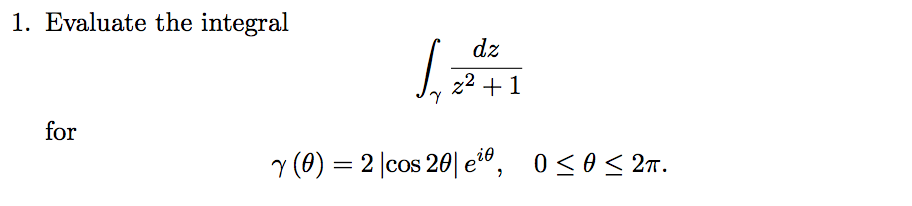
\includegraphics[width=1\textwidth]{cv-9-1}
\end{figure}
\end{question}
\begin{solution}
By drawing the contour on the complex plane, we observe that 
$\gamma$ forms 4 simple closed contours, for each direction of the axis.
We denote these contours as $\gamma_1$, $\gamma_2$, $\gamma_3$, and
$\gamma_4$ respectively in a counter-clockwise fashion. Observe that
$f(z) = \dfrac{1}{z^2+1}$ is singular at $z = \pm i$. $z = i$ belongs
to the interior of $\gamma_2$ contour, and $z = -i$ belongs to the
interior of $\gamma_4$ contour. By the Cauchy-Residue formula, we obtain
\eQb
\int_{\gamma_1} \dfrac{dz}{z^2+1} &=& 0 \\
\int_{\gamma_2} \dfrac{dz}{z^2+1} &=& 2\pi i 
\text{Res}_{z=i} \dfrac{1}{z^2+1}  \\
\int_{\gamma_3} \dfrac{dz}{z^2+1} &=& 0 \\
\int_{\gamma_4} \dfrac{dz}{z^2+1} &=& 2\pi i 
\text{Res}_{z=-i} \dfrac{1}{z^2+1}.\\
\eQe
As it can be written that
$f(z) = \dfrac{\phi(z)}{z-i}$, where $\phi(z) = \dfrac{1}{z+i}$,
the residue at $z = i$ is $\phi(i) = \dfrac{1}{2i}$. On the other hand,
as it can be written that
$f(z) = \dfrac{\phi(z)}{z+i}$, where $\phi(z) = \dfrac{1}{z-i}$, 
the residue at $z = -i$ is $\phi(i) = -\dfrac{1}{2i}$. Consequently, we have
\eQb
\int_{\gamma_2} \dfrac{dz}{z^2+1} &=& 2\pi i \dfrac{1}{2i} = \pi  \\
\int_{\gamma_4} \dfrac{dz}{z^2+1} &=& 2\pi i (-\dfrac{1}{2i}) = -\pi. \\
\eQe
Therefore, it follows that
\eQb
\int_{\gamma} \dfrac{dz}{z^2+1} &=& 
\int_{\gamma_1} \dfrac{dz}{z^2+1} + 
\int_{\gamma_2} \dfrac{dz}{z^2+1} +
\int_{\gamma_3} \dfrac{dz}{z^2+1} +
\int_{\gamma_4} \dfrac{dz}{z^2+1} \\
&=& 0.
\eQe
\hfill $\qed$
\end{solution}

\bigskip
\begin{question}[2]
\hfill
\begin{figure}[h!]
\centering
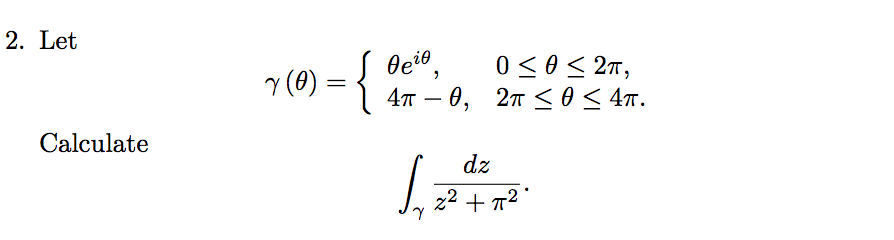
\includegraphics[width=1\textwidth]{cv-9-2}
\end{figure}
\end{question}
\begin{solution}
Observe that the function has isolated singularities at $z = \pm i \pi$. 
By observing the contour, we see that $i \pi$ lies outside of the contour,
as $\gamma(\dfrac{\pi}{2}) = \dfrac{\pi}{2}e^{i\frac{\pi}{2}} = 
i\dfrac{\pi}{2}$. On the other hand, $z = -i\pi$ lies on the interior of the
contour 
as $\gamma(\dfrac{3\pi}{2}) = \dfrac{3\pi}{2}e^{i\frac{3\pi}{2}} =
-\dfrac{3\pi}{2}i$. Hence, by the Cauchy Residue theorem, we have
\eQb
\int_{\gamma} \dfrac{dz}{z^2+\pi^2} &=& 2\pi i \text{Res}_{z=-i\pi} 
\dfrac{1}{z^2+\pi^2}.
\eQe  
As it can be written that $f(z) = \dfrac{\phi(z)}{z+i\pi}$, where
$\phi(z) = \dfrac{1}{z - i\pi}$, the residue at $z=-i\pi$ is 
$\phi(-i\pi) = -\dfrac{1}{2i\pi}$. Hence, it follows that
\eQb
\int_{\gamma} \dfrac{dz}{z^2+\pi^2} &=& 2\pi i (-\dfrac{1}{2i\pi}) \\
&=& -1. 
\eQe
\hfill $\qed$
\end{solution}

\begin{question}[3]
\end{question}
\begin{solution}
As we have $\lambda - z -e^{-\lambda} = 0$, we have 
\eQb
| \lambda - z | = e^{-\text{Re} z}. 
\eQe
Since $\text{Re} z > 0$, to satisfy the inequality, we must have
\eQb
| \lambda - z| < 1.
\eQe

\end{solution}

\bigskip

\begin{question}[4]
\end{question}
\begin{solution}

\end{solution}

\bigskip

\begin{question}[5]
\end{question}
\begin{solution}
\end{solution}



\end{document}


